\chapter{Introduction}

\section{Background}

Digital payments have become the default way of paying for goods and services. Card payments, online shopping, mobile banking and cross-border e-commerce now generate millions of transactions every day, and each of them is an opportunity for fraud. Financial crime is estimated to cost U.S. institutions alone more than 32 billion dollars each year \cite{uddin2026}. For banks and payment processors, detecting fraudulent transactions quickly and accurately is therefore both a financial and a trust problem.

Modern fraud detection systems (FDS) combine fixed business rules with machine-learning models that score each transaction and raise alerts for investigators \cite{dalpozzolo2018,alessi2026}. A large body of work has compared classifiers, ensembles and class-imbalance techniques on public data \cite{dang2021,abdelnaby2023,sohony2018,mienye2023}, and gradient boosted trees such as XGBoost have proved to be strong models for tabular fraud data \cite{amekoe2024,uddin2026}. Most of this work, however, studies the model at a single point in time: it is trained on a random sample of historical transactions and tested on another random sample from the same period.

Real systems do not work like that. A model is trained on the past and then used on the future, and the future does not stand still. Customers change their spending habits, merchants and products change, and fraudsters adapt their strategies to whatever the current model does not catch. This change in the relationship between transactions and fraud over time is known as concept drift \cite{pulicharla2019,kodakandla2024}. Under concept drift, a model that performed well at deployment slowly, and sometimes suddenly, becomes less accurate. Menezes and Filho, for example, found that the F1-score of graph neural network fraud detectors trained on the IEEE-CIS dataset fell by up to 40\% over the following weeks \cite{menezes2025}.

Fraud detection adds a second difficulty that most drift research does not consider: the true label of a transaction is not known when the model makes its decision. A fraud is usually confirmed only when the cardholder notices it and files a chargeback, and a legitimate transaction is only confirmed when the dispute window has passed. Dal Pozzolo et al. call this verification latency and show that it strongly affects how a fraud model can be updated \cite{dalpozzolo2018}, and Amekoe et al. showed that it changes which learning strategies work best \cite{amekoe2024}. In practice, the labels a system can learn from are often weeks old, which means that it can only notice that its performance has dropped long after the drop has happened.

Machine Learning Operations (MLOps) has emerged to handle exactly this kind of problem: keeping machine-learning models reliable after deployment through automated pipelines for training, versioning, monitoring and redeployment \cite{pulicharla2019,kodakandla2024}. A central MLOps practice is continuous training, where models are retrained either on a fixed schedule or when a monitoring signal indicates that the data has drifted \cite{pulicharla2019}. Recent research increasingly favours the second option, triggering retraining when statistical drift measures such as the Population Stability Index (PSI) or the Kolmogorov-Smirnov (KS) test exceed a threshold \cite{shakil2025,wong2025}. Whether such triggers actually track the performance of a fraud model when labels arrive late is, however, an open question. This thesis addresses that question and builds a framework around the answer.

In this thesis, a \textit{drift-aware} system is one that is aware of drift through its effect on the model: it tracks the performance of the deployed model on labels as they mature, and treats label-free drift measures as diagnostic information rather than as a reason to retrain. As the results will show, this distinction matters, because drift indicators alone can both miss real degradation and raise alarms about drift that does no harm.

\section{Motivation}

The first motivation for this study is the gap between how fraud models are evaluated in research and how they are used in practice. Many studies report near-perfect results on public credit-card datasets using random train-test splits and synthetic oversampling \cite{mienye2023}. Dang et al. showed that such results can be inflated when resampling is applied before splitting \cite{dang2021}, and a random split has a similar effect in time: the model is tested on transactions from the same period it was trained on, so concept drift is invisible. A fraud model that will be deployed on future transactions must be evaluated on future transactions.

The second motivation is that the decision of when to retrain a model is costly in both directions. Retraining too rarely leaves a degraded model in service and lets fraud through. Retraining too often wastes computing resources and, more importantly, increases the chance of deploying a bad model, for example one trained on incomplete or corrupted data. MLOps systems therefore need a policy that decides when retraining is actually necessary and a safeguard that decides whether a newly trained model may replace the one in service.

The third motivation is that recent work proposing drift-triggered retraining has been evaluated under conditions that favour it. Shakil et al. proposed a feature-drift indicator to decide when retraining is warranted, but tested it on drift that was artificially induced into non-fraud datasets \cite{shakil2025}. Wong and Perumal reported that an agentic, drift-triggered retraining scheduler outperformed weekly retraining, but on a single industrial dataset with injected drift \cite{wong2025}. Yelleti retrained fraud models only when a drift detector fired, but assumed that labels arrive immediately \cite{yelleti2025}. Shakil et al. themselves note that statistical drift does not always correspond to a change in model performance \cite{shakil2025}.

Finally, we are motivated by our own preliminary experiments on the IEEE-CIS dataset, which already challenge the common assumption. A LightGBM model trained once lost about a third of its weekly PR-AUC over the following months, yet the drift of its prediction scores stayed far below the usual alarm level, and only one of its ten most important features drifted noticeably. On a second dataset, Sparkov, we observed the opposite: strong input drift with almost no loss of accuracy. If drift detectors can both miss real decay and raise false alarms, a drift-aware system has to be designed around what drift detection can and cannot see. This is the perspective this thesis takes.

\section{Problem Statement}

We consider a fraud detection model deployed on a continuous stream of card transactions. Each transaction must be scored immediately, but its fraud label becomes available only after a label delay of several days to several weeks. Over time the distribution of transactions and the relationship between transaction features and fraud change. The operator of the system must decide, at regular intervals, whether to retrain the model, which data to retrain it on, and whether the retrained model is safe to put into service.

Existing approaches leave several parts of this problem unresolved:

\begin{enumerate}
  \item \textbf{Unrealistic evaluation.} Most fraud studies use random splits of static data, so they cannot show how performance evolves after deployment or how much retraining helps \cite{abdelnaby2023,mienye2023}.
  \item \textbf{Unverified retraining triggers.} Label-free drift measures such as PSI and KS are widely used to trigger retraining, but whether they track the performance of a fraud model has not been established on real, naturally drifting data \cite{shakil2025,wong2025}.
  \item \textbf{Ignored label delay.} Most retraining studies assume that labels are available immediately, although verification latency is a defining property of fraud detection \cite{dalpozzolo2018,amekoe2024}.
  \item \textbf{No fair comparison of retraining policies.} Scheduled and drift-triggered retraining are rarely compared under the same conditions, with tuned settings, uncertainty estimates and realistic label delay.
  \item \textbf{Unsafe model updates.} Automated retraining can deploy a model trained on corrupted labels or features; few frameworks test whether their safeguards actually stop such models.
  \item \textbf{Limited reproducibility.} Studies with realistic operating conditions often rely on private bank data \cite{dalpozzolo2018,somasundaram2019,aldaoud2025}.
\end{enumerate}

This thesis addresses these gaps through the following research questions:

\begin{itemize}[label={}, leftmargin=2em]
  \item \textbf{RQ1:} How does the performance of a fraud detection model evolve after deployment, and do label-free drift measures reflect that change?
  \item \textbf{RQ2:} How much does retraining improve performance, and how does label delay change that benefit?
  \item \textbf{RQ3:} Does drift-triggered retraining outperform scheduled retraining when both are tuned fairly and evaluated with realistic label delay?
  \item \textbf{RQ4:} Can an MLOps framework built on these findings sustain performance on a live stream and prevent faulty models from reaching production?
\end{itemize}

\section{Objective}

The aim of this research is to design and evaluate a drift-aware continuous learning MLOps framework for financial transaction fraud detection that can identify when a deployed model is becoming outdated, decide when retraining is actually necessary, and safely deploy a better retrained model without unnecessary retraining. The specific objectives are:

\begin{enumerate}
  \item To review existing research on fraud detection, concept drift, label delay, retraining strategies and MLOps, and identify the gaps this thesis addresses.
  \item To prepare three public fraud datasets, IEEE-CIS, Sparkov and BAF, for strictly time-ordered evaluation, without leakage from future transactions.
  \item To measure how a model trained once degrades over time, and whether label-free drift measures (PSI of features and of model scores) track that degradation.
  \item To simulate retraining strategies under label delays of 0 to 60 days: a static model, scheduled retraining on all past data or on a sliding window, and retraining triggered by drift in scores or by a drop in delayed-label performance.
  \item To compare these strategies with paired day-block bootstrap confidence intervals, walk-forward tuning of their settings and repeated training seeds.
  \item To implement an MLOps framework with delayed-label monitoring, a retraining policy, a promotion gate, a model registry, a scoring service and a monitoring dashboard.
  \item To test the safeguards of the framework by injecting realistic faults (corrupted labels, a chargeback outage and a feature unit bug) into its retraining jobs.
  \item To check whether the findings generalise by replicating the key experiments on the other two datasets.
\end{enumerate}

\section{Methodology in Brief}

The study follows the workflow shown in Figure \ref{fig:method}. It begins with a review of the literature on fraud detection, concept drift and MLOps, which identifies the gaps listed in the problem statement. Two public datasets are then prepared. IEEE-CIS, released by the IEEE Computational Intelligence Society and Vesta Corporation, contains 590,540 real e-commerce transactions over 182 days with a fraud rate of 3.5\% and has been used in recent drift and fraud studies \cite{menezes2025,uddin2026}. Sparkov contains about 1.8 million simulated card transactions over two years with a fraud rate of 0.5\%. Both are sorted by time and used without any random shuffling; per-card behaviour features for Sparkov are computed only from each card's earlier transactions, so that no information from the future leaks into the model.

\begin{figure}[htbp]
  \centering
  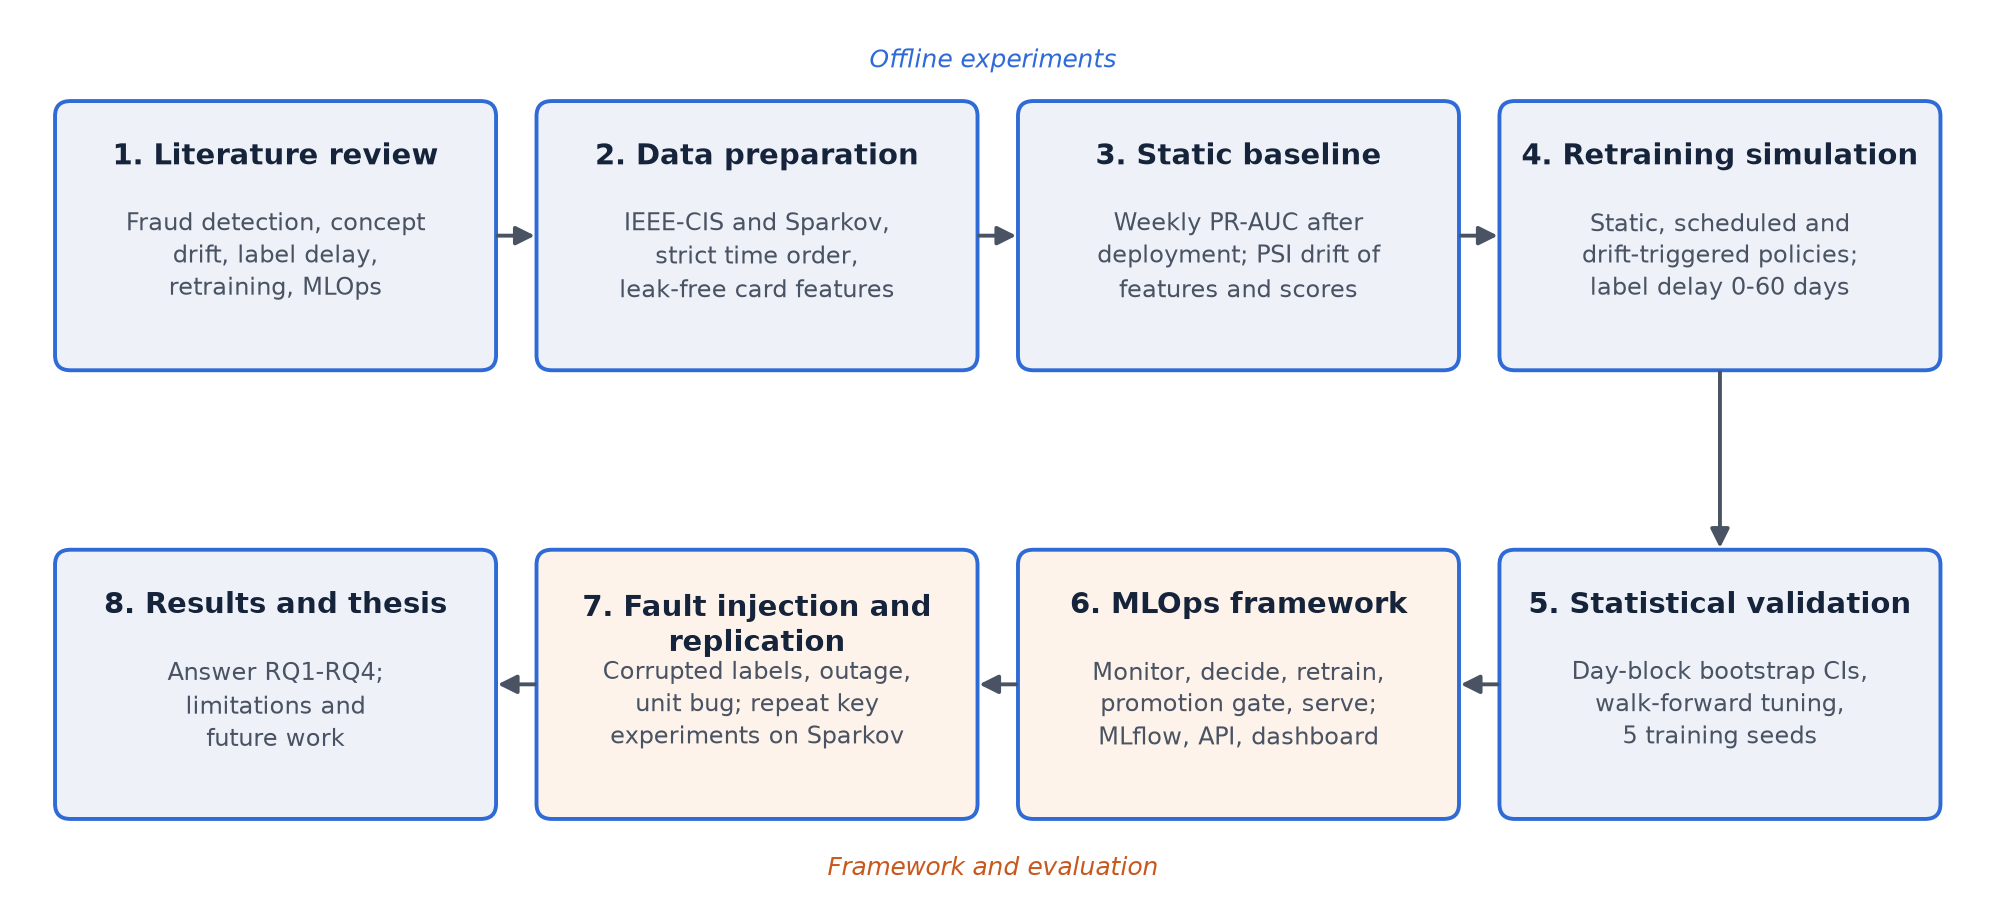
\includegraphics[width=\textwidth]{figures/methodology.png}
  \caption{Methodology of the study: from literature review and time-ordered data preparation to the retraining experiments, the framework and its evaluation}
  \label{fig:method}
\end{figure}

A LightGBM gradient boosted tree model is used throughout, because batch-trained boosted trees are strong, widely used models for tabular fraud data and remain competitive with incremental learners when labels are delayed \cite{amekoe2024}. The study first trains a static model and measures its weekly performance and the PSI drift of its features and scores over the following months. It then replays the later part of each dataset as a stream, week by week, and simulates the retraining strategies listed in the objectives, making labels available only after a chosen delay. PR-AUC is the main metric because fraud is rare and the precision of alerts matters most \cite{dalpozzolo2018}; results are averaged per week so that scores from different model versions are never pooled. Uncertainty is estimated with a paired bootstrap that resamples whole days, strategy settings are tuned walk-forward using only information available at the time, and the key comparisons are repeated with five training seeds.

The findings are then turned into a working framework, shown in Figure \ref{fig:loop}. Every week it measures the live model on labels that have become available, decides whether to retrain, trains a new model on a sliding window of recent labelled data, and promotes it only if a promotion gate confirms that it performs at least as well as the live model on data neither has seen. Models are versioned in MLflow, served through a FastAPI scoring service and tracked on a monitoring dashboard, following common MLOps practice \cite{pulicharla2019}. The framework is evaluated by replaying the stream end to end and by injecting faults into selected retraining jobs to test whether the promotion gate and performance safety net stop faulty models.

\begin{figure}[htbp]
  \centering
  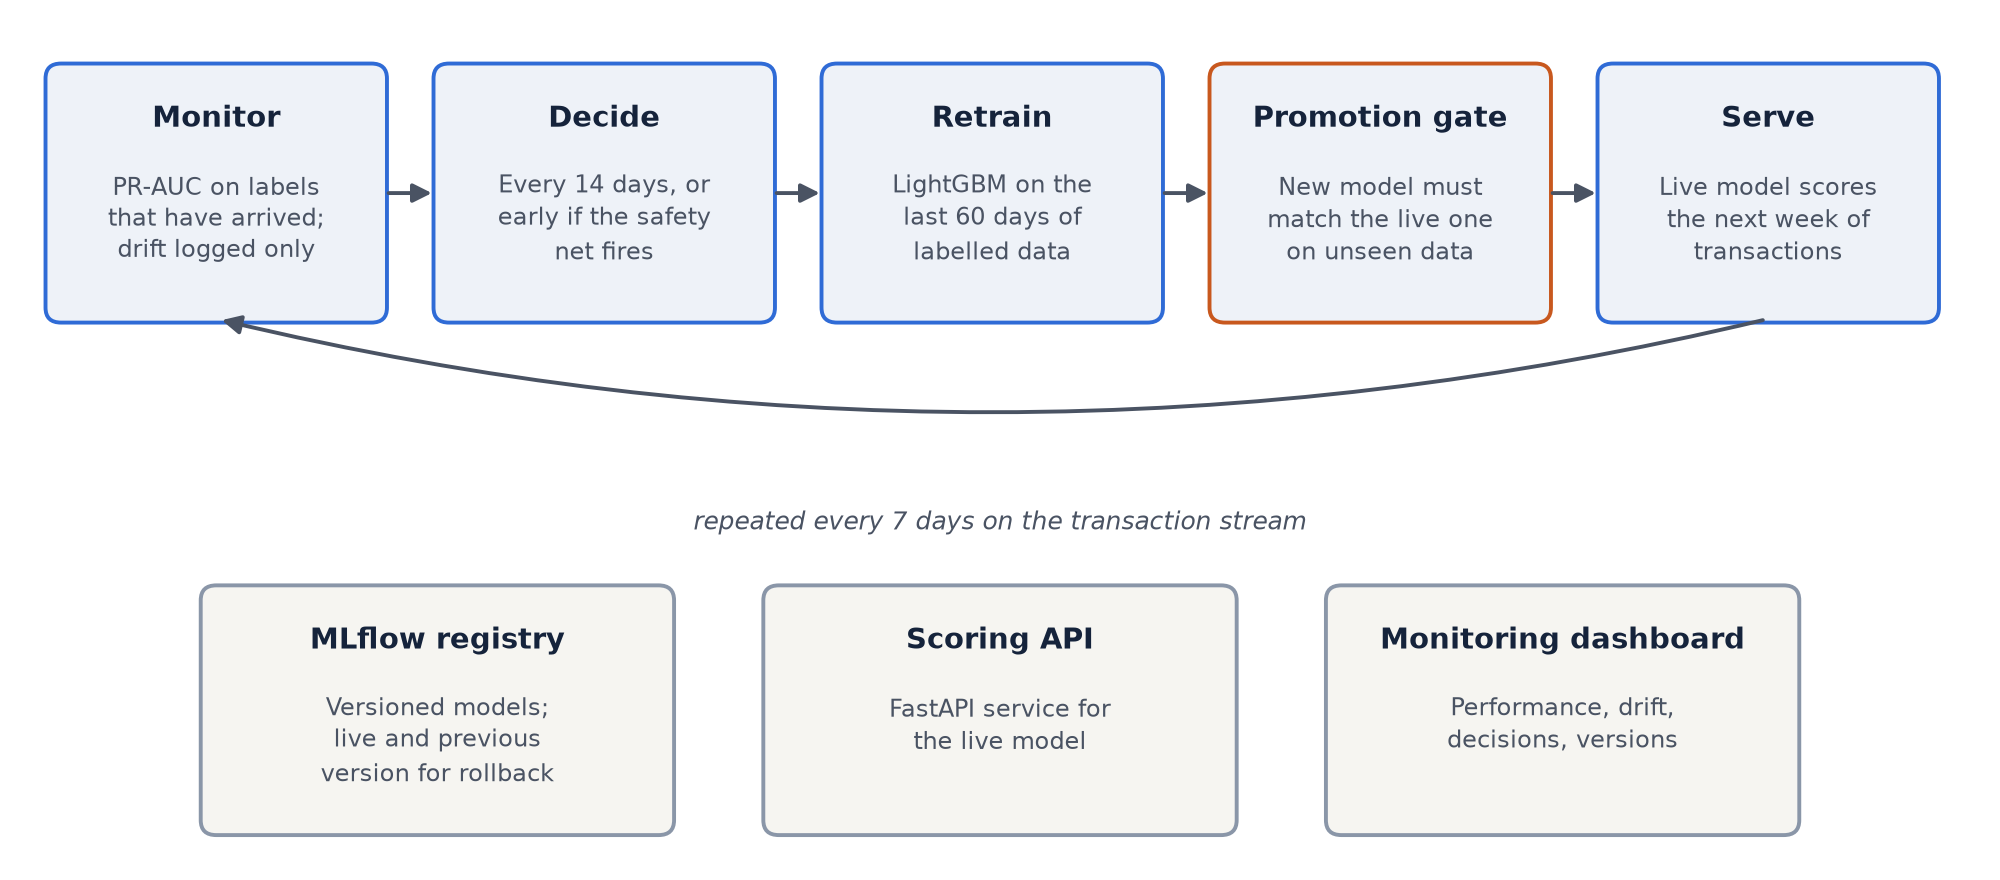
\includegraphics[width=\textwidth]{figures/framework_loop.png}
  \caption{The proposed continuous-learning loop, run every week on the transaction stream}
  \label{fig:loop}
\end{figure}

The experiments were run on IEEE-CIS and repeated on Sparkov and on the Bank Account Fraud (BAF) dataset. They show that drift indicators can miss real degradation under delayed labels, that a fixed retraining schedule is more reliable than drift-triggered retraining when labels are delayed, also at an equal retraining budget, and that the framework reproduces the offline results when replayed. The details are given in Chapters 4 and 5.

\section{Scopes and Challenges}

The study focuses on binary fraud detection for card transactions, where each transaction is scored as fraudulent or legitimate. Its scope is the post-deployment life of a model: how it degrades, when retraining is actually necessary, and how model updates can be made safe. It does not aim to find the best possible classifier, and it does not connect to a real bank or process real customer data. The main areas covered are:

\begin{enumerate}
  \item Time-ordered evaluation of fraud models on two public datasets.
  \item Analysis of performance decay and of label-free drift measures after deployment.
  \item Comparison of static, scheduled and drift-triggered retraining under label delay.
  \item Statistical validation with bootstrap confidence intervals, walk-forward tuning and repeated seeds.
  \item An MLOps framework with monitoring, retraining policy, promotion gate, model registry, scoring service and dashboard.
  \item Fault-injection testing of the framework's safeguards.
\end{enumerate}

The study also faces several challenges:

\begin{enumerate}
  \item \textbf{Label delay:} performance can only be measured on labels that have matured, so problems are always detected late.
  \item \textbf{Class imbalance:} frauds are rare (0.5\% to 3.5\% of transactions), which makes weekly performance estimates noisy and requires careful statistics.
  \item \textbf{Simulated deployment:} the stream is replayed from historical data, so live latency and real label-feed behaviour are not observed.
  \item \textbf{Limited datasets:} public fraud data with timestamps is scarce; IEEE-CIS covers only six months and Sparkov is simulated.
  \item \textbf{Anonymised features:} many IEEE-CIS features are masked, which limits the interpretation of which features drift and why.
  \item \textbf{Computational cost:} repeated retraining over long streams, several label delays and many policy settings requires hours of computation per experiment.
  \item \textbf{Generalisation:} results obtained with one model family and two datasets may not transfer to every institution or fraud type.
\end{enumerate}

Despite these challenges, the study can provide practical, evidence-based guidance on how fraud detection models should be maintained after deployment, and a reproducible open framework that implements it.
